\subsection{Deployment at Tier-2 sites}
The deployment of IPv6 at Tier-2 sites is still proceeding even after the
deadline expired at the end of 2018. It was decided not to
give the deadline a formal extension, but just to encourage all
remaining sites to complete the IPv6 deployment ``as soon as
possible'': the main motivations were that \emph{a)} sites behind
schedule were encountering objective difficulties and \emph{b)} the
most effective deadline would be imposed by the experiments
themselves, if they wished, for example, to require IPv6 for
production. This choice was confirmed by the steady progress observed
during 2019, as it can be seen in figure~\ref{fig:t2depl}.
\begin{figure}[h]
\centering
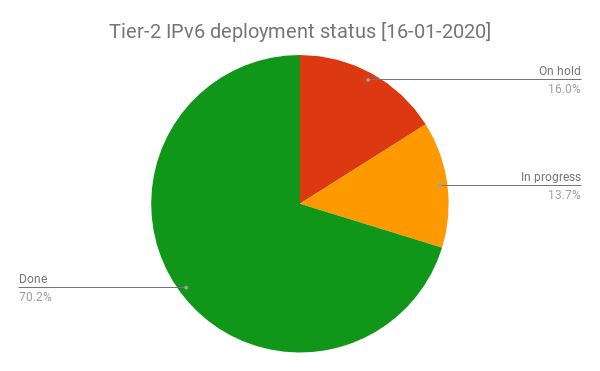
\includegraphics[width=6cm]{chart2}
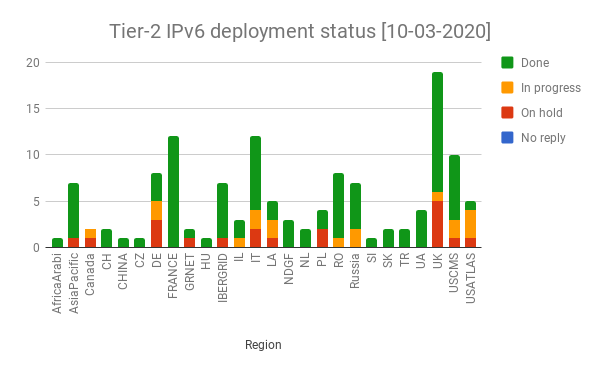
\includegraphics[width=6cm]{chart}
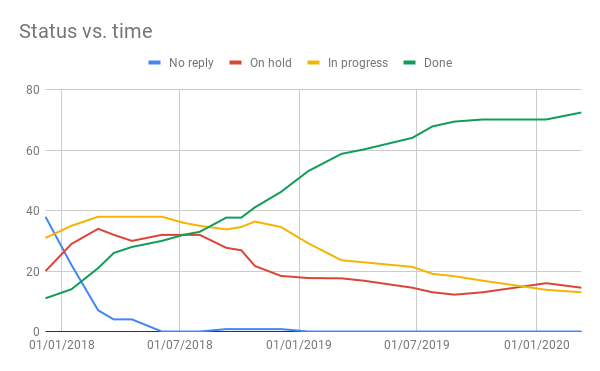
\includegraphics[width=6cm]{chart3}
\caption{(left) Tier-2 deployment status by site globally, (right) by region, and (bottom) time evolution}
\label{fig:t2depl}
\end{figure}

The time evolution of the site status shows a steady increase of the
number of sites that have deployed IPv6, until a more recent
slowdown. This is consistent with the hypothesis that the remaining
sites are those facing the biggest difficulties. 
The progress of each Tier-2 site is recorded  in a support tracking system with
 a separate ticket assigned to each site.
A detailed analysis
of these tickets shows that, in many cases, sites need to wait for the
IPv6 deployment on site, which often depends on people different from
the WLCG site staff. The fraction of the Tier-2 storage that is
accessible via IPv6 is shown in table~\ref{tab:t012stor} for each 
experiment, and significant differences are apparent.
%\begin{table}[h]
%\centering
%\caption{Fraction of Tier-1 and Tier-2 storage available over IPv6}
%\label{tab:t12stor}
%\begin{tabular}{lccccc}
%\hline
%& ALICE & ATLAS & CMS & LHCb & Global \\\hline
%Tier-1 storage & 78\% & 96\% & 100\% & 94\% & 96\% \\ 
%Tier-2 storage & 86\% & 59\% &  89\% & 75\% & 74\% \\\hline
%\end{tabular}
%\end{table}
Two experiments (ALICE and CMS) are very close to having all their
Tier-2 storage on IPv6, LHCb has little Tier-2 storage to begin with
due to their particular computing model and ATLAS is getting better,
but still far from the goal.

